\subsection{Transfer across generative models}\label{sec:joint-transfer}
We transfer both FM-trained correction networks to EDM and GAGA, fixing the correction weights and strengths. Each target retains its native source, backbone, and sampling schedule. Equation~\eqref{eq:endpoint-native-updates} converts the endpoint displacement into a noise-prediction correction.

\begin{figure}[!htbp]\centering
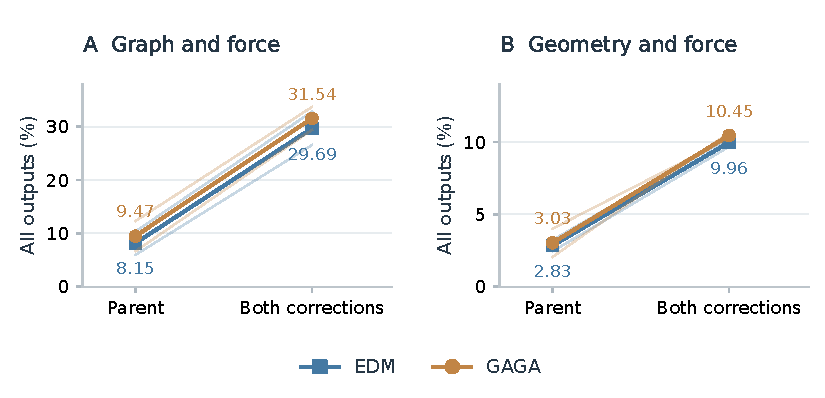
\includegraphics[width=\linewidth]{../research/figures/final_complete_v1/figures/geometric_transfer.pdf}
\caption{Direct transfer of both correction networks: (A) graph-and-force yield and (B) geometry-and-force yield. Bold lines show two-fit means and faint lines show individual fits. Each setting contains 2,048 attempts on 64 compositions, with the target source and backbone fixed and hydrogen readout disabled.}\label{fig:joint-transfer}\label{fig:seed-replication}
\end{figure}

Joint yield increases from 8.15 to 29.69\% for EDM and from 9.47 to 31.54\% for GAGA. Geometry-and-force yield increases from 2.83 to 9.96\% and from 3.03 to 10.45\%, respectively. Both metrics improve in both fits for each target. Together with the one-pass FM results in Figure~\ref{fig:source-head-ablation}, these experiments show direct correction-weight reuse across generative objectives within the shared EGNN architecture.

\paragraph{Physical-head transfer.}\label{sec:cross-head}\label{sec:seed-replication}
In the earlier five-pair study, transferring the physical head alone raised GAGA joint yield from 8.75 to 25.27\%, compared with 25.37\% using GAGA-trained heads. Across the three additional pairs, the mean transferred-head gain was 16.54 points (crossed 95\% interval $[12.66,20.67]$). Reverse transfer raised initial FM yield from 7.21 to 25.59\%. Appendix~\ref{app:seed-replication} reports all fits.

\paragraph{Source transfer and hydrogen readout.}
Retraining EDM and GAGA with harmonic corruption noise and adding the physical head alone gave joint yields of 0.00\% and 0.05\%, compared with native-parent yields of 8.15\% and 9.47\% (Appendix~\ref{app:joint-design-transfer}). In contrast, the successful weight transfers above preserve the target source. The optional hydrogen readout raised joint yield of the initial force-corrected generators to 26.33\% for FM and 25.74\% for GAGA; it is excluded from the main experiments.
